\documentclass[11pt]{article}
\usepackage{geometry}                % See geometry.pdf to learn the layout options. There are lots.
\geometry{letterpaper}                   % ... or a4paper or a5paper or ... 
%\geometry{landscape}                % Activate for for rotated page geometry
\usepackage[parfill]{parskip}    % Activate to begin paragraphs with an empty line rather than an indent
\usepackage{caption, subcaption} % enable subfigures
\usepackage{listings}
\renewcommand*{\refname}{\section{Referencer}} 
\usepackage[stable]{footmisc}
\usepackage{graphicx}
\usepackage{amssymb}
\usepackage{amsmath}
\usepackage{float}
\usepackage[utf8]{inputenc}
\usepackage{epstopdf}
\renewcommand*\contentsname{Indhold}
\renewcommand{\figurename}{Fig.}
\DeclareGraphicsRule{.tif}{png}{.png}{`convert #1 `dirname #1`/`basename #1 .tif`.png}
\graphicspath{ {/home/fall/Desktop/} }

%define paper title, author and date
%if date is empty, defaults to current date
\title{Automatisk tabeloprettelse og fejltjek til forsøgsresultater på Rigshospitalet\\
3. Delrapport - ProjDat 2014}
\author{Instruktor: Markus Lund Wittorf \\Gruppemedlemmer: \\ Mikkel Aleksander Høgh Rasmusen - 100888 \\ Mathias Fall Christensen - 020693 \\ Markus Visvaldis Ingemann Thieden - 170594}
\date{}

\begin{document}
\maketitle
\pagebreak
\tableofcontents
\pagebreak
\section{Litteraturreview}
\subsection{Brooks, F. P., No silver bullet}
\subsubsection{Hovedpunkter}
Artiklen beskriver en søgen efter en generel måde at løse problemer ifm. softwareudvikling; en så kaldt sølvkulge.\\
Først beskriver han problemet med en analogi over Aristoteles, hvori han deler problemerne op i to dele "essensen" og "uheld". Essensen er selve dataopbygningen og programarkitekturen. Essensen har følgende egenskaber:
\begin{itemize}
\item Kompleksitet
\item Overensstemmelse 
\item Omskiftlighed
\item Usynlighed.
\end{itemize}
Kompleksitet består i at software har utroligt mange stadier, og en meget kompleks opbygning, hvilket besværliggører kommunikationen mellem udviklere.\\
Eftersom software bliver udviklet af mennesker, er der mange holdninger til, hvordan programmer skal opbygges. Derfor er det vigtigt, at få sin software tilpasset med tidligere standarter, for at undgå yderligere kompleksitet.\\
Omskiftlighed gør det muligt at ændre softwaren efter udgivelse, hvilket er en funktion der er essentiel for enhver successful udgivelse, da hardware opdateres med jævne mellemrum.\\
Software er usynligt og uhåndgribeligt, fordi det er så komplekst. Man kan derfor ikke visualisere programmer, og de metoder der findes er overfladiske.\\
Uheld, som var den anden del af problemerne, er utilsigtet hændelser, hvor deres løsninger ofte bringer fremskridt. Uheld forekommer bl.a. når flere programmer skal snakke sammen.\\
Efterfølgende beskriver Brooks mulige håb for "sølvkulgen" - hvilke veje man kunne gå, for at få løst problemerne i softwareudvikling. Kunstig intelligens er en af de mulige løsninger. Han mener, at man lave en form for "expertsystem", som hjælper programøren med løsningen af eventuelle problemer, men han kan ikke komme med et gæt på, hvornår dette bliver en realitet.\\
 En anden mulighed er at købe færdiglavet programmer. Da der er en vækst af softwaredistributører, kan man spare penge på at købe færdiglavet software, i stedet for selv at udvikle det, da programmører er dyre i drift.\\ 
Den iterative proces beskrives også som en anden mulig "sølvkulge". Det er rigtig svært for en kunde at beskrive, præcist hvad det er de gerne vil have. Man kan løse dette problem ved at arbejde på, at lave tidlige prototyper, som kunden så kan forholde sig til. På denne måde angriber man essensen af softwaren, ved at udvikle og videreudvikle tilgangen til et problem.
\subsubsection{Tanker og spørgsmål}
Umiddelbart ville vi mene at artiklen er en anelse redundant. De problemer der bliver stillet op, er ganske vidst noget, der opstår inden for softwareudvikling, men når Brooks ikke selv kan komme på en ordenlig, realistisk løsning, falder artiklen til jorden. Bevares, det bliver nævnt, at den iterative proces er en god metode til at mindske antallet af problemer, og det er bestem også en holdning, vi i gruppen deler. Når det så er sagt, har Brooks nogle gode pointer i sin beskivelse af software - det han kalder "essencen". Selvfølgelig giver det god mening, at den software man udvikler, skal indrette sig efter software standarder og normer, og idéen om at, at din software skal være omskiftelig, har jo gjort at opdateringer til div. programmer udkommer så ofte som de gør. Det er måske det sidstnævnte, som vi vil bide os mest fast i, iforhold til artiklen, og det ligger klart og fast, at vi har tænkt os at benytte os at dette "råd".  


\pagebreak
\subsection{Ehn og Kyng, Cardboard computers}
\subsubsection{Hovepunkter}
Artiklen argumentererb for, at der er både fordele og ulemper ved "abstraherede" prototyper, eksemplificeret ved deres papcomputere. Fordelene opsummeres overordnet i fire punkter:
\begin{itemize}
\item "Hands-on experience"
\item Forståelighed
\item Lav omkostning
\item Sjovt (og dermed engagerende)
\end{itemize}
Forståelighed og "hands-on experience" går "hånd i hånd", da denne mockup metode er baseret på en kontrakt imellem designerne af mockup og de deltagende brugere. Denne kontrakt er i grunden en leg eller et "rollespil", da den kræver at deltagerne lever sig ind i den fantasi der er opstillet. Uden indlevelsen falder metoden til jorden. Hvis indlevelsen derimod er til stede kan brugeren få en kraftig fornemmelse af deltagelse i processen, og kan relatere deres "hands-on" oplevelser langt mere direkte, end hvis de skulle forholde sig abstrakt til det endelige programs teoretiske funktionaliteter.\\
Derudover medfører denne metode et intimt samarbejde mellem designere og brugere, og da det fysiske mockup kognitivt er så langt fra et computersimuleret mockup, risikerer brugeren ikke at forveksle tekniske problemer med designbeslutninger.\\
Endnu en fordel ved at lege med pap er, at det lægger op til en form for "super-rapid-prototyping". Når brugeren sidder med så fysiske manifestationer af funktionerne, lægger det op til eksperimentation og kritik på et andet niveau, end hvis de sad overfor en computerskærm, og de foreslåede ændringer kan implementeres og testes med det samme, blot ved at finde et andet dejligt stykke pap og en tusch.\\
Artiklen bevæger sig også ind på grænseområdet mellem den ovennævnte "pap-metode" og en mere "konservativ" mockup metodologi. Den argumenterer for, at efterhånden som man bevæger sig mod et mere "repræsentativt simulacrum" vil brugerens indlevelsesevne stige, især for brugere der kun deltager kort. Til gengæld begynder fordelene ved "klippe-klistre" metoden at forsvinde - det er for eksempel ikke lige så sjovt at sidde overfor et realistisk computermockup, som det er at sidde og lege med pap. Derved vil brugerens indlevelsesevne højnes på bekostning af blandt andet engagementet.\\
Man får ikke bonuspoint for at namedroppe Wittgenstein og Heidegger.

\subsubsection{Tanker og spørgsmål}
Artiklen er tydeligt præget af, at være skrevet i det sidste årtusinde. På trods af, at den sandsynligvis engang har været relevant (muligvis indenfor en anden sektor), er dens nuværende værdi allerhøjst tvivlsom. Nu om dage falder langt de fleste anvendelsesområder indenfor deres særkategori af "virksomheder der allerede har den påkrævede IT-infrastruktur", og hele paphistorien mister derfor en stor del af sin relevans. På trods af dette er der nogle meta-egenskaber ved designmetoden som med lidt god vilje kan overføres til den moderne verden. Vi har for eksempel designet et "tilsvarende" mockup i form af et billede af interfacet, som brugeren så kan kritisere. Mange af artiklens pointer kan dog ikke overføres ved denne overgang, som for eksempel den barnlige fornøjelse ved "legens sprog" og rollespillet, eller den rapid-prototyping man ville kunne få ud af, at brugeren blot kunne gribe det nærmeste stykke pap og tilføje en ny feature.

\pagebreak
\section{Delrapport}
\subsection{Abstract}
Vi laver en desktopapplikation til automatisk oprettelse af tabeller med henblik på forsøgs- resultatindsamling for Professor Lars Rasmussen fra anæstesi afd. på Rigshospitalet. Målet med projektet er en simplificere processen fra indledende forsøgsprotokol til klargjort tabel. Dette vil vi gøre ved at analysere protokollen, og automatisk oprette et dokument med de i protokollen angivne parametre. Outputtet er et dokument der kan læses af excel eller lignende programmer, som fungerer som en skabelon til  det specifikke forsøg. Derudover har vi en fejltjek-funktion, der kan undersøge om et udfyldt skema overholder specifikationerne. 


\subsection{IT-projektets formål og rammer}
\subsubsection{Functionality}
Opretter automatisk skemaer til forsøgsresultater ud fra protokoller. Tjekker indtastede værdier for varians fra angivne grænseværdier.
\subsubsection{Application domain}
Forskere på rigshospitalet.
\subsubsection{Conditions}
Programmet udvikles som led i projektkurset. Programmet vil blive anvendt til at reducere indtastningsfejl i forbindelse med forskningsresultater.
\subsubsection{Technology}
Programmet skrives i Java. Skrives til at være kompatibelt med rigshospitalets Windows-systemer.
\subsubsection{Objects}
Protokoller, skemaer og CRF'er (Case Report Files).
\subsubsection{Responsibility}
Automatisering af oprettelse af skemaer. Fejltjekning af indtastet data.

\subsection{Kravspecifikation for IT-løsningen}
\subsubsection{Funktionelle krav\footnote{Både funktionelle- og ikke-funktionelle krav er termer taget fra OOSE\cite{OOSE}}}
\begin{itemize}
  \item Skal i praksis kunne håndtere et stort antal parametre til oprettelse af tabeller.
  \item Skal kunne oprette et dokument med forsøgsparametre, som kan læses af Excel.
  \item Skal kunne "oversætte" en forsøgsprotokol og opfange parametre samt begrænsninger.
  \item Skal kunne sammenligne et udfyldt excelskema med forsøgsprotokollens krav, og advare brugeren hvis de ikke er overholdt.
\end{itemize}
\subsubsection{Ikke-funktionelle krav}
\begin{itemize}
  \item Skal kunne oprette tabeller hurtigere end manuel indtastning.
  \item Simpelt og overskueligt design.
  \item Skal være brugervenligt.
\end{itemize}
\pagebreak
\subsubsection{Use-case model}
\begin{figure}[H]
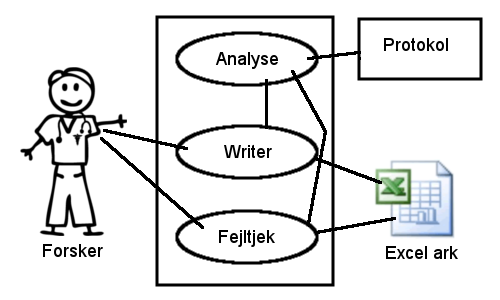
\includegraphics[scale=0.5]{usecase.png}
\caption{Use-case model}
\end{figure}
Forskeren kører Writer funktionen for at oprette et skema,
eller Fejltjek for at tjekke et skema.
Analyse indsamler information fra Protokollen.
Writer tager input fra Forskeren, henter information fra Analyse, og skriver Excel skemaet.
Fejltjek modtager parametre fra Forskeren, og sammenholder informationen fra Analyse med
skemaet angivet af Forskeren.
\subsubsection{Specificerede use-cases}
I opgavebeskrivelsen står der, at vi skal udforme 3 use-cases, men da vores program i realiteten kun skal kunne de ting, vi har beskrevet nedenfor, har det kun været muligt for os at lave disse to:\\
\begin{itemize}
\item[\textbf{USE CASE 1:}] Opret Excel Ark\\
\noindent\rule{14cm}{0.4pt}

\item [Participating actors:] \quad Forsker \\
\noindent\rule{14cm}{0.4pt}


\item [Flow of events:]
\begin{enumerate}
\item Forsker vælger stien for Protokol.
\item Forsker vælger stien for skema output.
\item Forsker indlæser protokollen.
\item Programmet læser værdier fra protokollen og viser dem i brugergrænsefladen
\item Forsker gennemlæser og bekræfter de indlæste værdier i brugergrænsefladen
\item Forsker opretter skemaet ved tryk på "Opret Skema"
\item Programmet skriver værdierne til en excel fil på den i skridt (2) valgte sti.
\end{enumerate}
\noindent\rule{14cm}{0.4pt}
\item[Entry condition:] Forskeren har startet programmet.\\
\noindent\rule{14cm}{0.4pt}

\item[Exit condition:]
\begin{itemize}
  \item Skemaet er blevet oprettet.
  \item Programmet afsluttes.
\end{itemize}
\noindent\rule{14cm}{0.4pt}
\item[Quality requirements:]
\begin{itemize}
\item Programmet skal oprette skemaet hurtigere end Forsker ville kunne gøre det på egen hånd.
\item Programmet skal finde alle relevante attributter og grænseværdier.
\end{itemize}

\noindent\rule{14cm}{0.4pt} \hfill \\

\end{itemize}
\begin{itemize}
\item[\textbf{USE CASE 2:}] Fejltjek Excel Ark\\
\noindent\rule{14cm}{0.4pt}
\item [Participating actors:] Forsker\\
\noindent\rule{14cm}{0.4pt}

\item [Flow of events:]
\begin{enumerate}
\item Forsker vælger stien for Protokol.
\item Forsker vælger stien for Excel Ark.
\item Forsker starter fejltjek ved tryk på "Kør tjek".
\item Programmet læser grænseværdier fra protokollen og sammenholder dem med værdierne i Excel arket.
\item Forsker aflæser fejlagtige værdier hvis de er tilstede, og foretager eventuelle rettelser.
\end{enumerate}
\item [Entry condition:] Forsker vælger "Tjek Skema" tabben.\\
\noindent\rule{14cm}{0.4pt}

\item [Exit condition:]
\begin{itemize}
\item Tjekket er kørt igennem.
\item Programmet afsluttes.
\end{itemize}
\noindent\rule{14cm}{0.4pt}

\item [Quality requirements:]
\begin{itemize}
\item Programmet skal vise en oversigt over alle værdier, der ikke ligger indenfor de i protokollen
angivne grænseværdier. \\
\end{itemize}
\noindent\rule{14cm}{0.4pt}

\end{itemize}

\subsubsection{Klassediagram}
\begin{figure}[h!]
\includegraphics[scale=0.5]{Klassediagram1.png}
\caption{Klassediagram}
\end{figure}
Forskeren bruger GUI'en til til at køre enten Write eller Fejltjek modulerne. Både Write og Fejltjek modulerne afhænger af analysedataen, som bliver lavet af Analysemodulet ud fra protokollen vha. PDFbox. Write modulet skriver (vha. JExcel Write) til et excel dokument. Fejltjek modulet læser et et excel dokument vha. JExcel Read og sender resultaterne videre til GUI'en, som viser dem til forskerne/brugerne.

\subsubsection{Sekvens-diagrammer}
Vi har lavet to sekvensdiagrammer, der passer til de to use-cases vi har beskrevet tidligere.
\begin{figure}[H]
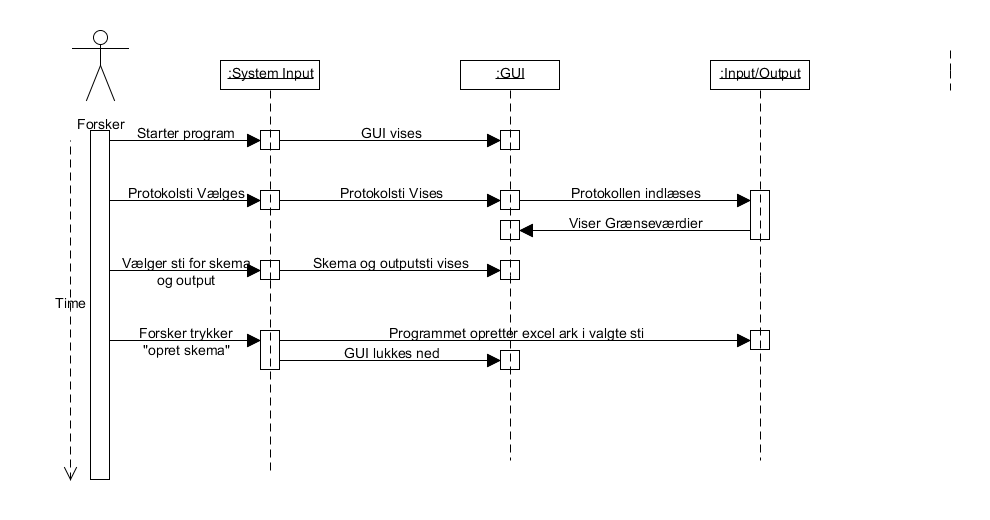
\includegraphics[scale=0.4]{Sekvensdiagram1} \hfill \\\\
\caption{Sekvensdiagram for Use-case nr.1}
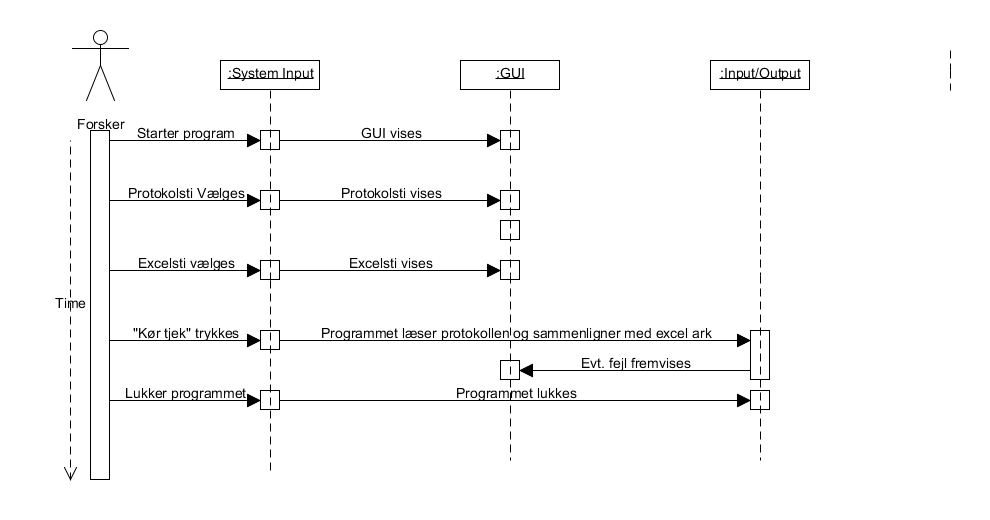
\includegraphics[scale=0.4]{Sekvensdiagram2}
\caption{Sekvensdiagram for Use-case nr.2}
\end{figure}
I fig. 3 er et sekvensdiagram over den første use-case, hvor forskeren benytter programmet til at oprette et skema ud fra en protokol.
I fig. 4 er et sekvensdiagram over den anden use-case, hvor forskeren benytter sig af den anden funktionalitet i programet til at tjekke et skema igennem for fejl.
\subsection{Systemdesign sammenfatning}
\subsubsection{System-design resume}
Da vi laver et program der skal kunne oprette excel dokumenter og læse PDF filer, har vi benyttet os af to ikke-standard Javapakker; PDFbox og JExcel\footnote{Kilderne kan findes på hhv. http://pdfbox.apache.org/ og http://jexcelapi.sourceforge.net/}. Metoderne i disse klasse danner stort grundlag for vores program, og vores opgave ligger i at bearbejde den data som PDFbox kan trække ud for os. Vi har 3 hoved moduler i programmet; \begin{itemize}

\item Analyse, der benytter sig af PDFbox 
\item Writer, der benytter sig af JExcel til at oprette et excel dokument 
\item Fejltjek, der benytter sig af begge pakker til at læse en protokol og et excel skema. 
\end{itemize} 
De sidstnævnte moduler er pt. ikke implementeret.
Analyse klassen er dog udarbejdet i en grov form (se punkt 2.7). 
\subsubsection{Udestående design- og implementationsopgaver}
Fejltjek og Writer klasserne er ikke blevet implementeren endnu, og det samme gælder GUI'en. Mht. til GUI'en, har vi dog en god idé om, hvordan den skal se ud jf. vores mockups. Fejltjek og Write afhænger i stor grad af Analyse klassen, så vi arbejder meget linært - vi kan ikke begynde på det næste modul, før den første er implementeret.\\I Analyse klassen, mangler vi en del der kan bearbejde den data der bliver udtrukket fra PDF'en. Dette har vi umidelbart tænkt os at gøre vha. Scanner klassen fra Javas standard bibliotek.

\subsection{Program- og systemtest}
Vores tests består hovedsageligt af at køre de enkelte moduler, for at tjekke deres funktionalitet. Det er ikke muligt at teste med brugere, før vores GUI er implementeret, men vi har dog planer om at fremvise en prototype af produktet til vores kunde. En kørsel af Analyse klassen er at finde under punkt 2.7.

\subsection{Brugergrænseflade og interaktionsdesign}
\begin{figure}[H]
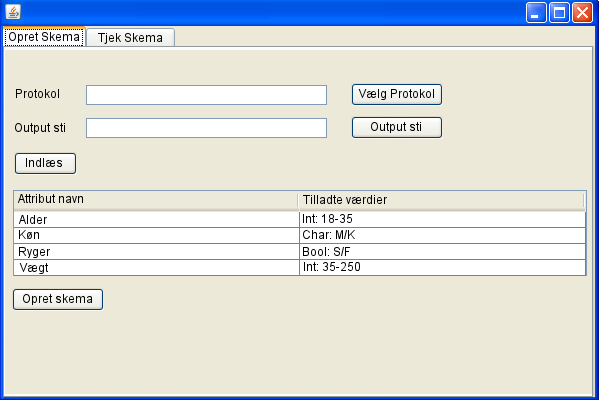
\includegraphics[scale=1]{osm.png}
\caption{Mockup af brugergrænseflade mht. Use-case nr.1}
\end{figure}
Her ses et mockup af vores brugergrænseflade. Protokolstien kan angives, og brugeren kan specificere hvor excelfilen skal oprettes. Tabellen viser en oversigt over de fundne attributter fra protokollen.\\
Som det ses, kan der navigeres mellem programmets to dele via fanerne i toppen af vinduet.
\begin{figure}[H]
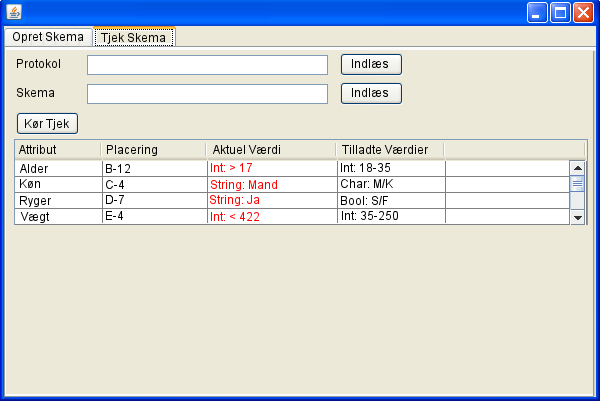
\includegraphics[scale=0.8]{mockup2.png}
\caption{Mockup af brugergrænseflade mht. Use-case nr.2}
\end{figure}

Dette er et mockup af den anden del af programmet. Her er idéen at der er blevet angivet et excel skema og den originale protokol, hvorefter der er blevet kørt et fejltjek. Tabellen viser evt. fejl eller afvigelser fra standard syntaks (f.eks. er der under køn blevet skrevet "Mand" i celle C-4, men protokollen har bedt om et input i form af M/K).
\pagebreak
\subsection{Versionsstyring}
På nuværende tidspunkt, har vi implementeret en grov version af klassen Analyse, der kan læse en PDF, og trække relevant data ud. 
Da vi pt ikke benytter os af github, kan vi ikke vise en commit-log, men vi har i sinde at begynde på det. I stedet har vi nedenfor den første implementation af Analyse-klassen, der giver et godt indblik i, hvad den skal gøre :
\begin{verbatim}
import java.io.*;
import org.apache.pdfbox.pdmodel.*;
import org.apache.pdfbox.util.*;
import java.util.regex.*;

public class Analyse {
   
    
   
 public static void main(String[] args){
 PDDocument pd;
 String att;
 try { 
         //  PDF fil der skal læses
         File input = new File(..(PDF sti angives her)..); 

         // StringBuilder opbevarer den udtrukkede tekst
         StringBuilder sb = new StringBuilder();
         pd = PDDocument.load(input);
         PDFTextStripper stripper = new PDFTextStripper();

         // Tilføjer text til StringBuilder
         sb.append(stripper.getText(pd));

         // Udtrækker relevant data fra pdf vha. regex.
         // Regex syntax kan findes her:
         // http://www.vogella.com/tutorials/JavaRegularExpressions/article.html
         // Leder efter linjer omsluttet af "//...//"
         Pattern p = Pattern.compile("//\\S+//");

         // Matcher, der leder i texten
         Matcher m = p.matcher(sb);

         while (m.find()){
             // group() metoden sætter teksten ind i variablen att.
             att = m.group();
             System.out.println(att);
         }

         if (pd != null) {
             pd.close();
         }
 } catch (Exception e){
         e.printStackTrace();
        }
     }
} 
\end{verbatim}
En kørsel af programmet med en protokol-PDF, vil finde og udsrive alle linjer omsluttet med "//...//", og som overholder en bestemt syntaks (e.g. //;Køn;Alder;Blodtype//). Herefter skal en anden del af klassen kunne separere attributterne (f.eks. hva. Scanner klassen fra Javas standard bibliotek) \\Den overordnede idé er, at det skal kunne være muligt at "browse" gennem fil stier via GUI'en, for at finde imput filen. Dette vil først være muligt når GUI'en er implementeret.

\subsubsection{Vigtigste ændringer}
Siden vores sidste aflevering, har vi ikke lavet nogle betydelige ændringer i vores kode. Vi forventer at have en endelig version af Analyse klassen, samt en grov implementation af Writer klassen klar indenfor den næste uge.
\subsection{Projektsamarbejdet}
Samarbejdet har fungeret fint indtil videre, så vi ser ingen grund til at ændre i denne.
Vi har fortsat tænkt os at holde møder på ugentlig basis, hvor kodning og evt. rettelser vil finde sted. Dog skal det nævnes at vi, på opfordring fra vores instruktor (og fordi det er et krav til opgaven) har tænkt os at begynde på at bruge github (se mere i afsnit 2.8.3).
\subsubsection{Hvad går godt?}
Vi er afklarede om målet for vores projekt.\\
Fremmødet har været upåklageligt.\\
Arbejdsmoralen er høj.\\
Samarbejdet fungerer stadig godt.
\subsubsection{Hvad går mindre godt?}
Vi er først lige nu ved at komme i gang med github.\\
Tidspresset er begyndt at tage til, hvilket kan have en negativ indflydelse på arbejdsmoralen.
\subsubsection{Effektivisering af udviklingsarbejde}
Vi vil begynde at bruge github, så vi kan arbejde uafhængigt af hinanden. Dette er ikke ensbetydende med at vi vil begynde at arbejde individuelt hele tiden, men hvis vi kan komme undgå at skulle mødes hver gang, vi skal kode, kan de i høj grad få øget tempoet på processen.
\begin{thebibliography}{9}

\bibitem{OOSE}
  Object-Oriented Software Engineering Using UML, Patters, and Java.
  \emph{Bernd Bruegge, Allen H. Dutoit}
  3rd Edition,
  2014.


\end{thebibliography}

\end{document}
